\documentclass[tikz,border=5pt]{standalone}
\usepackage{amsmath,amssymb,bm}
\usepackage{tikz}
\usetikzlibrary{arrows.meta,calc,positioning,fit,backgrounds,decorations.pathreplacing,shapes.geometric,quotes}
\definecolor{okBlue}{HTML}{4472C4}
\definecolor{okRed}{HTML}{C0504D}
\definecolor{okGreen}{HTML}{55A868}
\definecolor{okOrange}{HTML}{D98E04}
\definecolor{okPurple}{HTML}{7E57C2}
\definecolor{okGray}{HTML}{666666}
\definecolor{softBlue}{HTML}{EAF1FB}
\definecolor{softRed}{HTML}{F9ECEB}
\definecolor{softGreen}{HTML}{EDF7F0}
\tikzset{
  >={Latex[length=2.2mm,width=2.0mm]},
  every node/.style={font=\small},
  mathbox/.style={draw=black!55, rounded corners=2pt, very thick, fill=black!2, inner sep=5pt, align=center},
  chip/.style={draw=black!45, rounded corners=1.6pt, fill=black!1, inner sep=2pt, align=center},
  panel/.style={draw=black!55, rounded corners=2pt, line width=0.8pt},
  lightpanel/.style={draw=black!25, rounded corners=2pt, line width=0.5pt},
  flow/.style={-{Latex[length=2.3mm]}, line width=1.0pt, draw=black!70},
  thinflow/.style={-{Latex[length=1.9mm]}, line width=0.8pt, draw=black!55},
  faintcol/.style={draw=black!18, line width=0.6pt},
  reglabel/.style={font=\normalsize},
  srcA/.style={circle, draw=okBlue!70!black, fill=okBlue!15, minimum size=5.2pt, inner sep=0pt},
  srcB/.style={circle, draw=okRed!70!black, fill=okRed!15, minimum size=5.2pt, inner sep=0pt},
  tgtA/.style={circle, draw=okBlue!70!black, fill=okBlue!15, minimum size=5.2pt, inner sep=0pt},
  tgtB/.style={circle, draw=okRed!70!black, fill=okRed!15, minimum size=5.2pt, inner sep=0pt},
  crossdot/.style={diamond, draw=okOrange!80!black, fill=okOrange!85, minimum size=6pt, inner sep=0pt},
  kedge/.style={draw=okBlue!60!black, line width=0.9pt, opacity=0.50},
  triangleedge/.style={draw=okRed!75!black, line width=1.1pt, opacity=0.55},
  matching/.style={draw=okGreen!70!black, line width=1.8pt},
  absent/.style={draw=black!15, dashed, line width=0.55pt},
  qdata/.style={circle, fill=okGreen!75!black, draw=okGreen!55!black, minimum size=4.2pt, inner sep=0pt},
  qx/.style={rectangle, draw=okPurple!85!black, fill=white, minimum size=5.3pt, inner sep=0pt, line width=0.7pt},
  qz/.style={diamond, draw=okOrange!85!black, fill=white, minimum size=5.3pt, inner sep=0pt, line width=0.7pt},
  routeA/.style={draw=okBlue!85!black, line width=1.15pt, line cap=round, line join=round},
  routeB/.style={draw=okRed!85!black, line width=1.15pt, line cap=round, line join=round},
  access/.style={draw=black!40, densely dotted, line width=0.55pt},
  layA/.style={draw=okBlue!55!black, fill=okBlue!10, line width=0.7pt},
  layB/.style={draw=okRed!55!black, fill=okRed!10, line width=0.7pt},
  layBase/.style={draw=black!35, fill=black!5, line width=0.7pt},
  titleline/.style={font=\normalsize\bfseries},
  paneltag/.style={font=\bfseries\normalsize},
}

\begin{document}
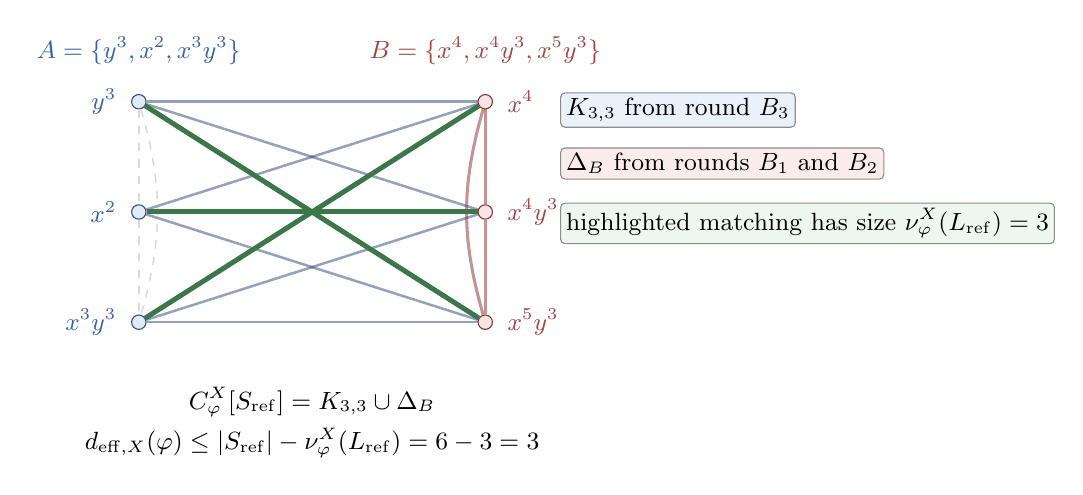
\begin{tikzpicture}[x=1cm,y=1cm]

  % Node positions
  \node[srcA] (a1) at (0.8,3.10) {};
  \node[srcA] (a2) at (0.8,1.70) {};
  \node[srcA] (a3) at (0.8,0.30) {};
  \node[srcB] (b1) at (5.20,3.10) {};
  \node[srcB] (b2) at (5.20,1.70) {};
  \node[srcB] (b3) at (5.20,0.30) {};

  \node[anchor=east, text=okBlue!85!black] at ($(a1)+(-0.16,0)$) {$y^3$};
  \node[anchor=east, text=okBlue!85!black] at ($(a2)+(-0.16,0)$) {$x^2$};
  \node[anchor=east, text=okBlue!85!black] at ($(a3)+(-0.16,0)$) {$x^3y^3$};
  \node[anchor=west, text=okRed!85!black] at ($(b1)+(0.16,0)$) {$x^4$};
  \node[anchor=west, text=okRed!85!black] at ($(b2)+(0.16,0)$) {$x^4y^3$};
  \node[anchor=west, text=okRed!85!black] at ($(b3)+(0.16,0)$) {$x^5y^3$};
  \node[text=okBlue!85!black, anchor=south] at (0.8,3.45) {$A=\{y^3,x^2,x^3y^3\}$};
  \node[text=okRed!85!black, anchor=south] at (5.2,3.45) {$B=\{x^4,x^4y^3,x^5y^3\}$};

  % faint absent A-internal edges
  \draw[absent] (a1)--(a2);
  \draw[absent] (a2)--(a3);
  \draw[absent] (a1) to[bend left=16] (a3);

  % K_{3,3} from B3
  \foreach \u/\v in {a1/b1,a1/b2,a1/b3,a2/b1,a2/b2,a2/b3,a3/b1,a3/b2,a3/b3}{\draw[kedge] (\u)--(\v);}  

  % triangle in B from B1,B2
  \draw[triangleedge] (b1)--(b2);
  \draw[triangleedge] (b2)--(b3);
  \draw[triangleedge] (b1) to[bend right=16] (b3);

  % matching
  \draw[matching] (a1)--(b3);
  \draw[matching] (a2)--(b2);
  \draw[matching] (a3)--(b1);

  % annotations
  \node[chip, fill=softBlue, anchor=north west] at (6.15,3.22) {$K_{3,3}$ from round $B_3$};
  \node[chip, fill=softRed, anchor=north west] at (6.15,2.52) {$\Delta_B$ from rounds $B_1$ and $B_2$};
  \node[chip, fill=softGreen, anchor=north west] at (6.15,1.82) {highlighted matching has size $\nu_\varphi^X(L_{\mathrm{ref}})=3$};

  \node[anchor=north] at (3.00,-0.40) {$C_{\varphi}^{X}[S_{\mathrm{ref}}]=K_{3,3}\cup \Delta_B$};
  \node[anchor=north] at (3.00,-0.92) {$d_{\mathrm{eff},X}(\varphi)\le |S_{\mathrm{ref}}|-\nu_\varphi^X(L_{\mathrm{ref}})=6-3=3$};
\end{tikzpicture}
\end{document}
